\documentclass[a4paper,11pt]{article}
\usepackage{lmodern}
\renewcommand*\familydefault{\sfdefault}
\usepackage{sfmath}
\usepackage[utf8]{inputenc}
\usepackage[T1]{fontenc}
\usepackage[italian]{babel}
\usepackage{indentfirst}
\usepackage{graphicx}
\usepackage{tikz}
\usepackage{listings}
\newcommand*\circled[1]{\tikz[baseline=(char.base)]{
		\node[shape=circle,draw,inner sep=2pt] (char) {#1};}}
\usepackage{enumitem}
\usepackage[left=2cm, right=2cm, bottom=3cm]{geometry}
\frenchspacing

\newcommand{\num}[1]{#1}

% Macro varie...
\newcommand{\file}[1]{\texttt{#1}}
\renewcommand{\arraystretch}{1.3}
\newcommand{\esempio}[2]{
\noindent\begin{minipage}{\textwidth}
\begin{tabular}{|p{8cm}|p{8cm}|}
	\hline
      \textbf{\file{input.txt}} & \textbf{\file{output.txt}}\\
	\hline
	\tt \small #1 &
	\tt \small #2 \\
	\hline
\end{tabular}
\end{minipage}
}

% Dati del task
\newcommand{\gara}{Esame Algoritmi 2018-07-25}
\newcommand{\nome}{La ragnatela di Tecla}
\newcommand{\nomebreve}{tecla}

\begin{document}
% Intestazione
\noindent{\Large \gara}
\vspace{0.5cm}

\noindent{\Huge \textbf \nome~(\texttt{\nomebreve})}

% Descrizione del task
\section*{Descrizione del problema}

Ape Maya \`e rimasta intrappolata in un nodo della tela di Tecla, un ragno molto temuto tra le api dell'alveare. Tecla si affretta ad afferrarla ma, quando giunge su quel nodo, si accorge di non avere appetito, e dice ``BLEAH''. Va detto che l'appetito dei ragni \`e molto particolare: ogni volta che percorrono un filamento della loro rete, essi invertono lo stato del loro stomaco tra ``SLURP'' e ``BLEAH''. Tecla deve quindi farsi un giretto nella rete sperando di tornare da Maya in stato ``SLURP''.

La tela di Tecla è composta da $N$ nodi (numerati da $0$ a $N-1$) connessi tra loro da $M$ filamenti. Tecla e Ape Maya all'inizio si trovano entrambe nel nodo $0$, e ogni filamento può essere attraversato da Tecla in entrambe le direzioni. Aiuta Tecla ad individuare una passeggiata funzionale al buon appetito!


% Input
\section*{Dati di input}
\newcommand{\inputfile}{\texttt{input.txt}}

Il file \inputfile{} è composto da $M+1$ righe, contenenti:
\begin{itemize}[nolistsep,itemsep=2mm]
\item Riga $1$: gli interi $N$ ed $M$, il numero di nodi e di filamenti della tela.
\item Riga~$i$, con $i=2\ldots M+1$: due interi separati da spazio $u$, $v$; dove $u$ e $v$ identificano i due nodi ai capi del filamento $i$-esimo.
\end{itemize}

% Output
\section*{Dati di output}
\newcommand{\outputfile}{\texttt{output.txt}}

Il file \outputfile{} deve essere composto da due righe, contenenti:
\begin{itemize}[nolistsep,itemsep=2mm]
\item Riga $1$: il numero di spostamenti $L$ che Tecla deve compiere nella sua passeggiata.
\item Riga $2$: $L+1$ numeri separati da uno spazio, di cui il primo e l'ultimo devono essere $0$ (nodo di partenza e di arrivo), e gli altri sono i nodi come visitati da Tecla nell'ordine (e possono avere ripetizioni).
\end{itemize}


% Esempi
\section*{Primo Esempio di input/output}
\esempio{
3 3

0 1

1 2

2 0
}{
3
  
0 2 1 0
}

In questo \textbf{primo caso di esempio}, la tela di Tecla \`e come nella figura seguente, dove il percorso da seguire \`e evidenziato in rosso:
\begin{center}
	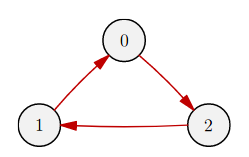
\includegraphics[scale=0.5]{asy_tecla/tecla1.png}
\end{center}



\section*{Secondo Esempio di input/output}
\esempio{
8 12

0 1

1 2

2 3

3 0

2 4

3 4

4 5

5 6

6 7

7 0

0 5

6 3
}{
7
  
0 5 6 3 4 2 3 0
}

In questo \textbf{secondo caso di esempio}, la tela e il percorso sono:
\begin{center}
	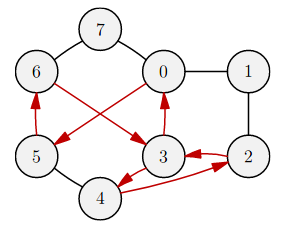
\includegraphics[scale=1.7]{asy_tecla/tecla2.png}
\end{center}


% Assunzioni
\section*{Assunzioni}

\begin{itemize}[nolistsep, itemsep=2mm]
    \item $ 1 \leq M, N \leq 1\,000\,000$.
    \item In ogni filamento, $u \neq v$ e sono entrambi compresi tra $0$ e $N-1$.
    \item Tecla prende avvio in stato ``BLEAH'' dal nodo~$0$.
    \item Si garantisce l'esistenza di una soluzione: Ape Maya \`e spacciata!
\end{itemize}

% Subtasks
\section*{Subtask}
\begin{itemize}
\item \textbf{Subtask 1 [0 punti]:} i due esempi del testo.
\item \textbf{Subtask 2 [10 punti]:} esiste il collegamento tra ogni coppia di nodi.
\item \textbf{Subtask 3 [10 punti]:} il nodo $0$ \`e adiacente ad ogni altro nodo. Ed almeno un ulteriore collegamento \`e presente.
\item \textbf{Subtask 4[20 punti]:} ogni nodo ha grado $2$.
\item \textbf{Subtask 5 [20 punti]:} $N \leq 10$.
\item \textbf{Subtask 6 [10 punti]:} $M,N \leq 100$.
\item \textbf{Subtask 7 [10 punti]:} $M,N \leq 1\,000$.
\item \textbf{Subtask 8 [20 punti]:} nessuna restrizione, $M,N \leq 1\,000\,000$.
\end{itemize}


\end{document}
